\chapter{RF-Score-v3: binding affinity prediction}

\section{Abstract}

There is a growing body of evidence showing that machine learning regression results in much more accurate structure-based prediction of protein-ligand binding affinity. Such pre-diction is a requirement for docking methods in that it is the basis for discriminating between active and inactive molecules or optimising the potency of a ligand against a target. However, despite their proven advantages, machine-learning scoring functions are still not widely applied. This seems to be due to insufficient understanding of their properties and the lack of user-friendly software implementing them.

Here we present a study where the accuracy of Vina, arguably the most commonly-used docking software, is strongly improved by following a machine learning approach. We also analyse the factors that are responsible for this improvement and their generality. Most importantly, with the help of a pro-posed benchmark, we demonstrate that this improvement will be larger as more data becomes available for training Random Forest models, as regression models implying additive functional forms do not improve with more training data. We dis-cuss how the latter opens the door to new opportunities in scoring function development. In order to facilitate the translation of this advance to enhance structure-based molecular design, we provide software to directly re-score Vina-generated poses and thus strongly improve their predicted binding affinity. The rescoring software is freely available at http://istar.cse.cuhk.edu.hk/rf-score-3.tgz.

This was a collaborative project with Pedro J. Ballester from European Bioinformatics Institute, Cambridge, United Kingdom, and Cancer Research Center of Marseille, Marseille, France. It was published in the \textit{Proceedings of the 11th International Meeting on Computational Intelligence Methods for Bioinformatics and Biostatistics (CIBB)} on 26 June 2014 \citep{1433}.

\section{Introduction}

\citep{1399} rescoring docked poses is also seen in protein-protein docking using machine learning techniques. T-PioDock, a framework for detection of a native-like docked complex 3D structure. T-PioDock aims at supporting the identification of near-native conformations from 3D models produced by docking software by scoring those models.
\citep{1389} A rotation-translation invariant molecular descriptor of partial charges and its use in ligand-based virtual screening
\citep{1389} For an extensive reference on molecular descriptors, cf. [10]. The DRAGON software [14] can compute thousands of such descriptors.
\citep{1400} QuBiLS-MIDAS: a parallel free-software for molecular descriptors computation based on multilinear algebraic maps
http://www.talete.mi.it/products/dragon\_description.htm Dragon 6 calculates 4885 molecular descriptors.

\citep{1423} comparison of confirmed inactive and randomly selected compounds as negative training examples in support vector machine-based virtual screening
\citep{1404} The influence of negative training set size on machine learning-based virtual screening

\citep{1377} Random generalized linear model: a highly accurate and interpretable ensemble predictor
\citep{1418} Predicting COPD status with a random generalized linear model

\citep{1426} Comparative Assessment of Scoring Functions on an Updated Benchmark: 1. Compilation of the Test Set
\citep{1411} Comparative Assessment of Scoring Functions on an Updated Benchmark: 2. Evaluation Methods and General Results

Molecular docking is a key computational technique in structural bioinformatics and structure-based molecular design. Docking predicts the preferred conformations and binding strength of a ligand molecule, typically a small organic molecule, as bound to a protein pocket. Such prediction is necessary to discriminate between molecules that bind and those that do not bind to a target of interest (i.e. those molecules with high affinity for the target and those with an affinity so low that does not permit stable binding). Docking is not only useful to anticipate whether a ligand binds tightly to a target, but also to understand how it binds. The latter can be helpful to improve the potency and selectivity of binding. Docking applications include structure-based virtual screening \citep{455,1383,1448}, drug lead optimisation \citep{1385}, polypharmacology prediction \citep{1449,1450}, drug repositioning \citep{1384}, binding pocket prediction \citep{384,1217}, human variation prediction \citep{1451}, protein function prediction \citep{1386} and target druggability assessment \citep{1472}.

Operationally, docking has two stages: predicting the position, orientation and conformation of a molecule when docked to the target's binding site (pose generation), and predicting how strongly the docked pose of such putative ligand binds to the target (scoring).  The single most important limitation of docking is the traditionally low accuracy of the scoring functions (SFs) that predict the strength of binding. Classical SFs assume a predetermined theory-inspired functional form for the relationship between the numerical features that describe the complex and its predicted binding affinity. There are three types of classical SFs: force-field \citep{1461,1462,959}, empirical \citep{1463,1464,1465,1466} and knowledge-based \citep{1467,1468,1469,1470}. Each type follows a different philosophical approach to SF development, as explained elsewhere, e.g. \citep{579}. However, it is important to note that these three types are mathematically equivalent in that a predetermined functional form is imposed to vertebrate the SF (in almost all classical SFs, the assumed functional form is additive). Furthermore, like empirical SFs, most modern force-field and knowledge-based SFs weight their constituent terms by fitting experimental binding data \citep{579}. Figure \ref{rfscore3:ClassicalScoringFunctions} illustrates the mathematical equivalence of three popular classical SFs as sums of data-weighted energetic contributions to binding. $K_j$ is the total number of protein atoms of type $j$ and $L_i$ is the total number of ligand atoms of type $i$ in the considered complex. An atom type is defined according to atomic number and in some cases also using the calculated protonation state (e.g. hydrogen bond donors). The additive terms may additionally impose interatomic distance and angle constraints between neighbouring atoms of the considered types (e.g. hydrogen bonding terms).

\begin{figure}
\centering
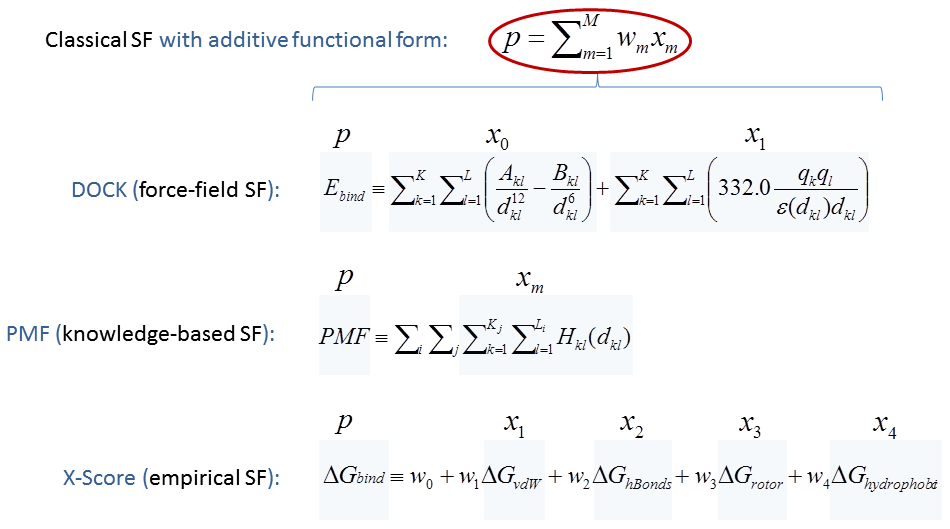
\includegraphics[width=\linewidth]{../rfscore3/ClassicalScoringFunctions.png}
\caption{Mathematical equivalence of classical scoring functions as sums of data-weighted energetic contributions to binding.}
\label{rfscore3:ClassicalScoringFunctions}
\end{figure}

Recently, machine-learning SFs have been shown \citep{564} to be much more accurate than classical SFs at binding affinity prediction. This improvement is due to two factors. The first is circumventing the assumed functional form of classical SFs, which is learnt instead in an entirely data-driven manner in machine-learning SFs. This was to be expected as it is well-known that individual free energy terms may not be additive \citep{1471,1416}. Second, research on classical SFs has focused on increasingly detailed modelling of contributions to binding, but it has now been established that a more precise description of protein-ligand complexes does not generally lead to more accurate prediction of binding affinity \citep{1370}. This study has resulted in an expected set of structural descriptors leading to improved performance when allied with a sufficiently flexible regression model. Machine-learning SFs have been misclassified as knowledge-based SFs \citep{1373,1372} or empirical SFs \citep{1305}, but these are fundamentally different from either type because of not imposing a fixed functional form on the relationship between structural and binding data. This distinction between machine-learning and classical SFs has important consequences in practice, as it will be analysed in section 3.4. Despite being a recent development, there are already successful prospective applications of machine-learning SFs. RF-Score \citep{564} has recently been used \citep{1281} to discover a large number of innovative binders of antibacterial DHQase2 targets. To facilitate its use, RF-Score  has now been incorporated into a user-friendly large-scale docking webserver for prospective virtual screening, available at http://istar.cse.cuhk.edu.hk/idock \citep{1362}. On the other hand, a machine-learning SF called MD-SVR has been generated and applied \citep{1452} to guiding the optimisation of known Akt1 kinase inhibitors. The derivatives highlighted by MD-SVR were synthesised and all of them exhibited moderate to good inhibitory activities.

This innovative methodology has however raised a few concerns. For example, the use of oversimplified features in the original version of RF-Score has been pointed out as problematic \citep{1453}, although no empirical evidence was provided in support of this claim and this version actually achieved high hit rates in prospective virtual screening \citep{1281}. The superior performance of RF-Score was highlighted by \citep{774}, who nevertheless attribute it to the characteristics of the most widely-used benchmark. This was subsequently demonstrated not to be the case \citep{908}. Still, there seem to be some concerns that the applicability domain of machine-learning SFs would be somehow more restrictive than that of classical SFs. Lastly, \citep{1372} claimed that the application of machine-learning SFs is limited by their tendency to overfit training data and their alleged difficulty in providing an immediate physical interpretation of the results.

In this paper, we show that one can construct a machine-learning SF from a classical SF to have the same applicability domain and interpretability capabilities while greatly improving its ability to predict binding affinity. This will be shown with AutoDock Vina \citep{595} as the classical SF. Furthermore, we will also address the remaining criticisms supported by numerical experiments. Finally, the growing importance of machine-learning SFs will be demonstrated in the context of a purposely-built new bench-mark by analysing how their performances improve with the in-crease of structural and binding data used for training.

\section{Methods}

This section introduces four SFs building upon AutoDock Vina, two benchmarks to evaluate performance of these SFs and the performance metrics that will be used to this end.

\subsection{AutoDock Vina (model 1)}

The AutoDock series \citep{597,596,595} is the most cited docking software by the research community, with over 8,000 citations to date between these three publications (source: Google Scholar). As the successor of AutoDock 4 \citep{596}, AutoDock Vina \citep{595} significantly improved the average accuracy of the binding mode predictions, while running two orders of magnitude faster with multithreading. Vina was an exciting development, not only because of its remarkable pose generation performance in terms of both effectiveness and efficiency, but also because it is an open source tool and is among the most accurate classical SFs for binding affinity prediction.

Like all classical SFs, Vina assumes a predetermined functional form. In this case, Vina's score for the $k$th conformer ($e_k$) is calculated as:

\begin{equation}
\label{rfscore3:e_k}
e_k=\frac{e_{k,inter}+e_{k,intra}-e_{1,intra}}{1+w_6N_{rot}}
\end{equation}

Now because studies on binding affinity prediction are benchmarked on co-crystallised ligands to avoid confounding factors, there is only one conformer per molecule (k=1) and thus the intramolecular contribution cancels out giving:

\begin{equation}
\label{rfscore3:e_1}
e_1=\frac{e_{1,inter}}{1+w_6N_{rot}}
\end{equation}

where

\begin{equation}
\label{rfscore3:e_1_inter}
e_{1,inter}=w_1Gauss1_1+w_2Gauss2_1+w_3Repulsion_1+w_4Hydrophobic_1+w_5HBonding_1
\end{equation}

\begin{equation}
\label{rfscore3:w}
\mathbf w=(-0.035579,-0.005156,0.840245,-0.035069,-0.587439,0.05846)
\end{equation}

$e_1$ is the predicted free energy of binding reported by the Vina software when re-scoring the structure of a protein-ligand complex. The values for the six weights were found by Ordinary Least Squares (OLS) using a nonlinear optimisation algorithm as it has been the case in related force-field SFs \citep{1454}, although this process was not detailed in the original publication \citep{595}. Unlike other classical SFs, Vina is not exactly a sum of energy terms because $w_6\neq0$, although it is quasi-linear since $1 + w_6N_{rot}$ takes values close to 1 for most protein-ligand complexes. As usual, e.g. \citep{1362}, the predicted free energy of binding in kcal/mol units is converted into pKd with $pK_d=-0.73349480509e_1$ in order to compare to binding affinities ($pK_d$ or $pK_i$). Expressions and further details for the five $e_k$, inter terms can be found in \citep{595,1362}.

\subsection{MLR::Vina (model 2)}

This is a Multiple Linear Regression (MLR) model using the six unweighted Vina terms as features. In order to make the problem amenable to MLR, we made a grid search on the w6 weight and there-after ran MLR on the remaining five weights as explained in the next section. Note that the use of MLR as the regression model implies an additive functional form and hence MLR::Vina is a classical SF. It adopts the philosophy of empirical SFs.

\subsection{RF::Vina (model 3)}

While Vina's ability to predict binding affinity is among the best provided by classical SFs, it is still limited by the assumption of a functional form. To investigate the impact of this modelling assumption, we used Random Forest (RF) to implicitly learn the functional form from the data. A RF is an ensemble of many different decision trees randomly generated from the same training data \citep{1309}. Instead of using all features, RF selects the best data split at each node of the tree from a typically small number (mtry) of randomly chosen features. In regression problems, the RF prediction is given by arithmetic mean of all the individual tree predictions in the forest. Here we built a RF model with the six Vina features using the default number of trees (500) and values of the mtry control parameter from 1 to all 6 features. The selected model will be that with the mtry value providing the lowest RMSE on a subset of training data known as the Out-of-Bag (OOB) data. Further details on RF model building in this context can be found in \citep{564}. Other machine learning techniques can of course be applied to this problem, e.g. SVR \citep{1295}, although this is out of the scope of the study.

\subsection{RF::VinaElem (model 4)}

This is the model described in the previous section with an expanded set of features (42 features once the 36 RF-Score features are added to the six Vina features). For a given random seed, a RF for each mtry value from 1 to 42 is built and that with the lowest RMSE on OOB data is selected as the SF. Briefly, to calculate RF-Score features, atom types are selected so as to generate features that are as dense as possible, while considering all the heavy atoms commonly observed in PDB complexes (C, N, O, F, P, S, Cl, Br, I). As the number of protein-ligand contacts is constant for a particular complex, the more atom types are considered the sparser the resulting features will be. Therefore, a minimal set of atom types is selected by considering atomic number only. Furthermore, a smaller set of interaction features has the additional advantage of leading to computationally faster SFs. RF-Score features are defined as the occurrence count of intermolecular contacts between elemental atom types $i$ and $j$:

\begin{equation}
\label{rfscore3:x_ij}
x_{ij}=\sum_{k=1}^{K_j}\sum_{l=1}^{L_i}H(d_{cutoff}-d_{kl})   \mathbf x=\{x_{ij}\}\in N^36
\end{equation}

where $d_{kl}$ is the Euclidean distance between the $k$th protein atom of type $j$ and the $l$th ligand atom of type $i$ calculated from a structure; $K_j$ is the total number of protein atoms of type $j$ and $L_i$ is the total number of ligand atoms of type $i$ in the considered complex; $H$ is the Heaviside step function that counts contacts within a $d_{cutoff}$ neighbourhood. Full details on RF-Score features are available at \citep{564}.

\subsection{The PDBbind benchmark}

Using a predefined training and test sets, where other SFs had previously been tested, has the advantage of minimising the risk of using a benchmark complementary to the presented SF. There are many examples of benchmarks to validate generic SFs \citep{1455,1456,571,1457}. Here we use the PDBbind benchmark \citep{1313}, arguably the most widely-used for binding affinity prediction of diverse complexes. This benchmark is based on the 2007 version of the PDBbind database, which contains a particularly diverse collection of protein-ligand complexes (1300 protein-ligand complexes with their corresponding binding affinities), assembled through a systematic mining of the entire PDB. The PDBbind benchmark essentially consists of testing the predictions of SFs on the 2007 core set, which comprises 195 diverse complexes with measured binding affinities spanning more than 12 orders of magnitude, while training in the remaining 1105 complexes in the refined set. In this way, a set of protein-ligand complexes with measured binding affinity can be processed to give two non-overlapping data sets, where each complex is represented by its feature vector $\mathbf x_i$ and its binding affinity $y_i$ (this includes both pKd and pKi measurements, which are henceforth referred to as pKd for simplicity):

\begin{equation}
\label{rfscore3:D_train}
D_{train}=\{y_i,\mathbf x_i\}_{i=1}^{1105}
\end{equation}

\begin{equation}
\label{rfscore3:D_test}
D_{test}=\{y_i,\mathbf x_i\}_{i=1106}^{1300}
\end{equation}

\begin{equation}
\label{rfscore3:y}
y=pK_d=-\log_{10}K_d
\end{equation}

This benchmark has the advantage of permitting a direct comparison against the performance of 16 classical SFs on the same test set \citep{1313}. These 16 classical SFs include five scoring functions in the Discovery Studio software version 2.0 from Accelrys: LigScore \citep{1466}, PLP \citep{1467}, PMF \citep{1468}, Jain \citep{1473} and LUDI \citep{1463}, five scoring functions (D-Score, PMF-Score, G-Score, Chem-Score, and F-Score) in the SYBYL software version 7.2 from Tripos, GlideScore \citep{1465} in the Schrödinger software version 8.0 from Schrödinger, three scoring functions in the GOLD software version 3.2 from the CCDC: GoldScore \citep{1474}, ChemScore \citep{1464} and ASP \citep{1469}, and two standalone scoring functions released by academic groups: DrugScore \citep{1470,1475} and X-Score version 1.2 \citep{573}. Several of these scoring functions had different versions or multiple options, including LigScore (LigScore1 and LigScore2), PLP (PLP1 and PLP2), and LUDI (LUDI1, LUDI2, and LUDI3) in Discovery Studio; GlideScore (GlideScore-SP and GlideScore-XP) in the Schrödinger software; DrugScore (Drug-ScorePDB and DrugScoreCSD); and X-Score (HPScore, HMScore, and HSScore). For simplicity, the authors that tested all these SFs on the PDBbind benchmark \citep{1313} only re-ported the best performance of the version/options of each SF. Furthermore, we can add to the comparison other classical SFs that have subsequently been tested on this benchmark: IMP::RankScore \citep{987} in \citep{1370}, HYDE2.0::HbondsHydrophobic \citep{1458}, Phoenix \citep{576}, Cyscore \citep{1372}, HotLig \citep{1459} and DSX\textsuperscript{CSD} \citep{1460}. Many machine-learning SFs have also been tested on this benchmark, which are however not relevant for the goals of this study and hence not included.

\subsection{The 2013 blind benchmark}

We propose a new benchmark mimicking a blind test to provide a more realistic validation than the PDBbind benchmark, where higher performance is to be expected due to the protocol that generates this partition \citep{908}. The new test set will comprise all the structures in the 2013 release of the PDBbind refined set that were not already in the 2012 release (i.e. the new 382 protein-ligand complexes added in 2013), whereas the 2012 refined set will be used for training. This is hence conducted as a blind test in that only data available until a certain year is used to build the SF that predicts the binding affinities of 2013 complexes as if these had not been measured yet. In addition to that in this benchmark, we define three more training sets to account for the structural and binding data available in the public domain at three previous times (these three previous PDBbind releases were selected so that there is approximately the same number of complexes between consecutive releases). In this way, one can use these four partitions sharing the same test set to study how SF performance varies with training data set size. Table \ref{rfscore3:partitions} shows the data partitions. Partition 1 is the PDBbind benchmark. Refined02 means the 2002 release of the PDBbind refined set, whereas refined07\\core07 means the complexes left in refined07 after removing those in core07. By construction of each partition, there are no complexes in common between any training set and test set pair (i.e. there is no overlap between both sets and hence each test set complex is new data not seen in model training). The parameter values of each model for each of these five training sets are provided in the supplementary information.

\begin{table}
\caption{Summary of the data set partitions.}
\label{rfscore3:partitions}
\begin{tabular}{clrlr}
\hline
Partition & Training set & N & Test set & N\\
\hline
1 & refined07$\backslash$core07 & 1105 & core07               & 195\\
2 & refined02         &  792 & refined13$\backslash$refined12 & 382\\
3 & refined07         & 1300 & refined13$\backslash$refined12 & 382\\
4 & refined10         & 2059 & refined13$\backslash$refined12 & 382\\
5 & refined12         & 2897 & refined13$\backslash$refined12 & 382\\
\hline
\end{tabular}
\end{table}

One may argue that an additional partition is necessary, where all training complexes that are in some way similar to any of the test complexes are removed. Nevertheless, in practice, a test set will contain really few complexes of this type. Therefore, we would be depriving the SFs of the most relevant training data, which would actually be available, without good reason, leading to unrealistically low performance for all SFs. This point has already been discussed elsewhere \citep{908}.

\subsection{Performance measures}

As usual \citep{1313}, performance will be measured by the Standard Deviation (SD), Root Mean Square Error (RMSE), Pearson correlation (Rp) and Spearman rank-correlation (Rs) between predicted and measured binding affinity. SD and RMSE, despite providing essentially the same SF rankings, are included to permit comparison to previously-tested scoring functions on this benchmark. Both reflect the ability of the scoring function to report an accurate binding affinity value, with RMSE being a more realistic measure. Rs shows how well it can rank bound ligands according to binding strength. Rp simply shows how linear the correlation is and thus it is a less relevant indicator of the quality of the prediction.

\section{Results and discussion}

\subsection{The impact of overfitting on RF performance}

It has been recently claimed \citep{1372} that the tendency of machine-learning SFs to overfit training data is a weak point limiting their application. This is a surprisingly common misconception, whereby a less overfitted model is regarded as necessarily better than a more overfitted model. The latter implicitly assumes that the impact of overfitting will be the same for different classes of regression models. Nevertheless, some models, e.g. RF, are robust to overfitting in the sense that this has a low impact on its generalization ability. For example, we trained MLR::Vina and RF::Vina on the same 1105 complexes and use them to predict the binding affinity of the 195 test set complexes (partition 1 in Table \ref{rfscore3:partitions}). MLR::Vina performed better on the training set than on the test set (SD=1.73 vs SD=1.88, respectively), which suggests that classical SFs only have a small degree of overfitting. In contrast, RF::Vina's performance was much better on the training set than on the test set (SD=0.60 vs SD=1.61, respectively), which evidences that RF significantly over-fits training data. However, the large performance gain of RF::Vina over MLR::Vina on the test set (SD =1.61 vs SD=1.88, respectively) makes clear that RF::Vina is substantially more accurate than MLR::Vina regardless of overfitting. Therefore, overfitting cannot be used to anticipate the relative performance of two different models on a test set and hence it is necessary to measure the true impact of overfitting on the compared models. An intuitive explanation of how a model can be robust to overfitting is provided in the Supplementary Information.

Next, partition 5 from Table \ref{rfscore3:partitions} is used to provide further evidence that overfitting is not a weak point limiting the application of RF-based SFs. This test set is composed by 382 complexes, which as that from partition 1 also contains complexes that are very different among themselves. The set is subdivided into five equally-sized new sets and the operation is repeated ten times to provide 50 different test sets with 76 or 77 complexes each. Thereafter, we evaluate MLR::Vina and RF::VinaElem on each test set and plot the resulting SD errors in Figure \ref{rfscore3:Models24SD}. If overfitting was a problem with RF, a highly variable difference in performance between both models would have been observed, with the less overfitted model being often better than the more overfitted model. By contrast, not once MLR::Vina outperforms RF::VinaElem. 

\begin{figure}
\centering
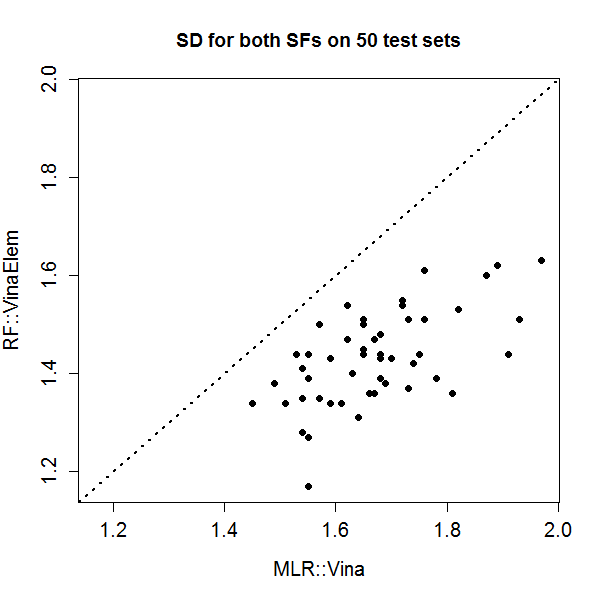
\includegraphics[width=\linewidth]{../rfscore3/Models24SD.png}
\caption{MLR::Vina and RF::VinaElem, both trained on the same 2897 complexes, compared on 50 test sets by their SD errors.}
\label{rfscore3:Models24SD}
\end{figure}

\subsection{Machine-learning SFs are remarkably more accurate than empirical SFs}

Table \ref{rfscore3:trn1105tst195} compares the performance of RF::VinaElem against that of 21 classical SFs and two sample baselines. Section 2.5 specifies the latter as well as some other classical SFs that only reported some of the performance measures, which hence cannot be included in the full comparison in Table \ref{rfscore3:trn1105tst195}: DSX\textsuperscript{CSD}::All \citep{1460} (Rp=0.609) and HotLig \citep{1459} (Rs=0.609).

\begin{table}
\caption{Performance of 22 SFs on the PDBbind benchmark as measured by Pearson's correlation coefficient (Rp), Spearman's correlation coefficient (Rs) and standard deviation (SD) of the difference between predicted and measured binding affinity. In addition, NHA is the performance of a linear regression model with the number of heavy atoms of the ligand as only variable that serves as a performance baseline and MWT is second baseline that uses the molecular weight of the ligand instead of NHA as the variable.}
\label{rfscore3:trn1105tst195}
\begin{tabular}{lrrr}
\hline
Scoring function & Rp & Rs & SD\\
\hline
RF::VinaElem               & 0.803 & 0.798 & 1.42\\
Cyscore                    & 0.660 & 0.687 & 1.79\\
X-Score::HMScore           & 0.644 & 0.705 & 1.83\\
HYDE2.0::HbondsHydrophobic & 0.620 & 0.669 & 1.89\\
DrugScoreCSD               & 0.569 & 0.627 & 1.96\\
SYBYL::ChemScore           & 0.555 & 0.585 & 1.98\\
AutoDock Vina              & 0.554 & 0.608 & 1.99\\
DS::PLP1                   & 0.545 & 0.588 & 2.00\\
GOLD::ASP                  & 0.534 & 0.577 & 2.02\\
SYBYL::G-Score             & 0.492 & 0.536 & 2.08\\
DS::LUDI3                  & 0.487 & 0.478 & 2.09\\
DS::LigScore2              & 0.464 & 0.507 & 2.12\\
GlideScore-XP              & 0.457 & 0.435 & 2.14\\
DS::PMF                    & 0.445 & 0.448 & 2.14\\
GOLD::ChemScore            & 0.441 & 0.452 & 2.15\\
NHA baseline               & 0.431 & 0.517 & 2.15\\
PHOENIX                    & 0.616 & 0.644 & 2.16\\
MWT baseline               & 0.418 & 0.496 & 2.17\\
SYBYL::D-Score             & 0.392 & 0.447 & 2.19\\
DS::Jain                   & 0.316 & 0.346 & 2.24\\
IMP::RankScore             & 0.322 & 0.348 & 2.25\\
GOLD::GoldScore            & 0.295 & 0.322 & 2.29\\
SYBYL::PMF-Score           & 0.268 & 0.273 & 2.29\\
SYBYL::F-Score             & 0.216 & 0.243 & 2.35\\
\hline
\end{tabular}
\end{table}

While it has been claimed \citep{1372} that empirical SFs have similar accuracy than machine-learning SFs, the results in Table \ref{rfscore3:trn1105tst195} clearly demonstrate that this is not the case. Indeed, the improvement introduced by RF::VinaElem over the best classical SFs is much larger than what has recently been considered acceptable for publication. For instance, Cyscore was shown to outperform the best classical SF, X-Score::HMScore, by only 0.04 in SD error \citep{1372}. By contrast, RF::VinaElem improves these SFs by 0.37 and 0.41 in this study, respectively (i.e. 9 and 10 times larger SD error reduction). Figure \ref{rfscore3:StandardDeviations} plots these differences. The + signs correspond to the classical SFs, the x sign is the SD of RF::VinaElem and the dotted vertical line is the SD of the NHA baseline.

\begin{figure}
\centering
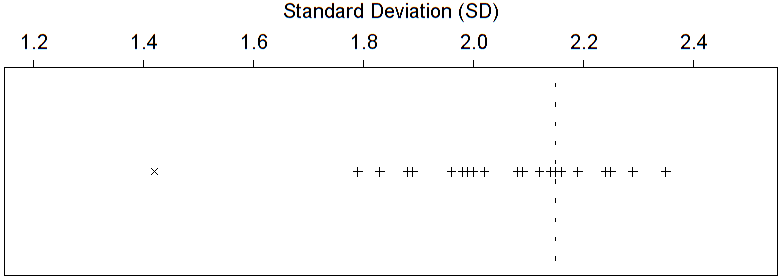
\includegraphics[width=\linewidth]{../rfscore3/StandardDeviations.png}
\caption{SD errors on the PDBbind benchmark for 22 scoring functions.}
\label{rfscore3:StandardDeviations}
\end{figure}

\subsection{Improvement of AutoDock Vina using RF}

RF::VinaElem is the result of two improvements over Vina: using RF on the six Vina features to circumvent the need of a functional form (model 3) and combining the latter with an expanded set of features (i.e. model 4 using the 36 RF-Score features added to the six from Vina). Figure \ref{rfscore3:partition1stat} shows their performance on PDBbind benchmark, with RF::VinaElem greatly improving Vina by -0.90 in RMSE, -0.57 in SD, +0.249 in Rp and +0.190 in Rs. A linear regression model with molecular weight of the ligand as only variable was trained and tested on the sets and obtained RMSE=2.16, SD=2.17, Rp=0.418 and Rs=0.496.

\begin{figure}
\centering
\subfloat[AutoDock Vina.]
{
  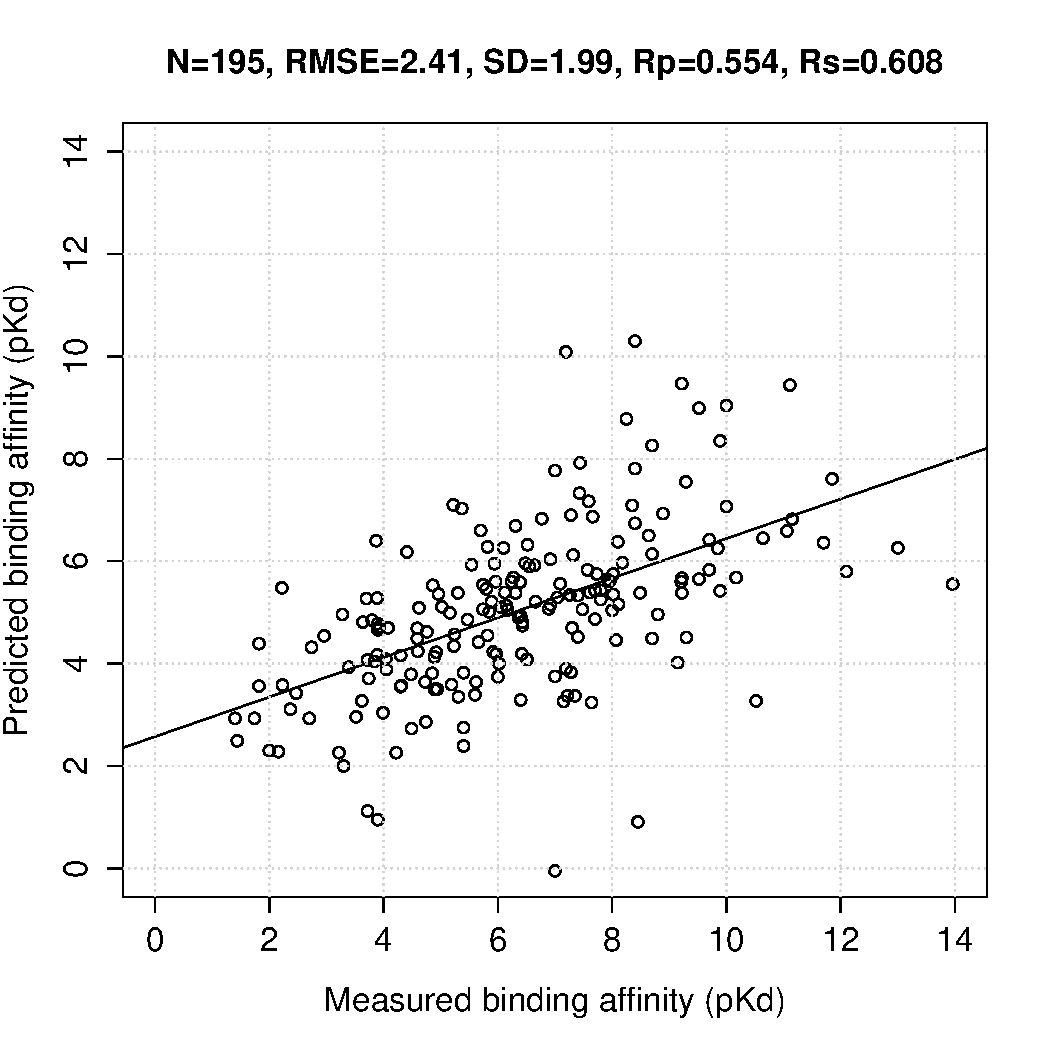
\includegraphics[width=0.48\linewidth]{../rfscore3/model-1-set-1-pdbbind-2007-tst-yp.pdf}
}
\subfloat[RF::VinaElem.]
{
  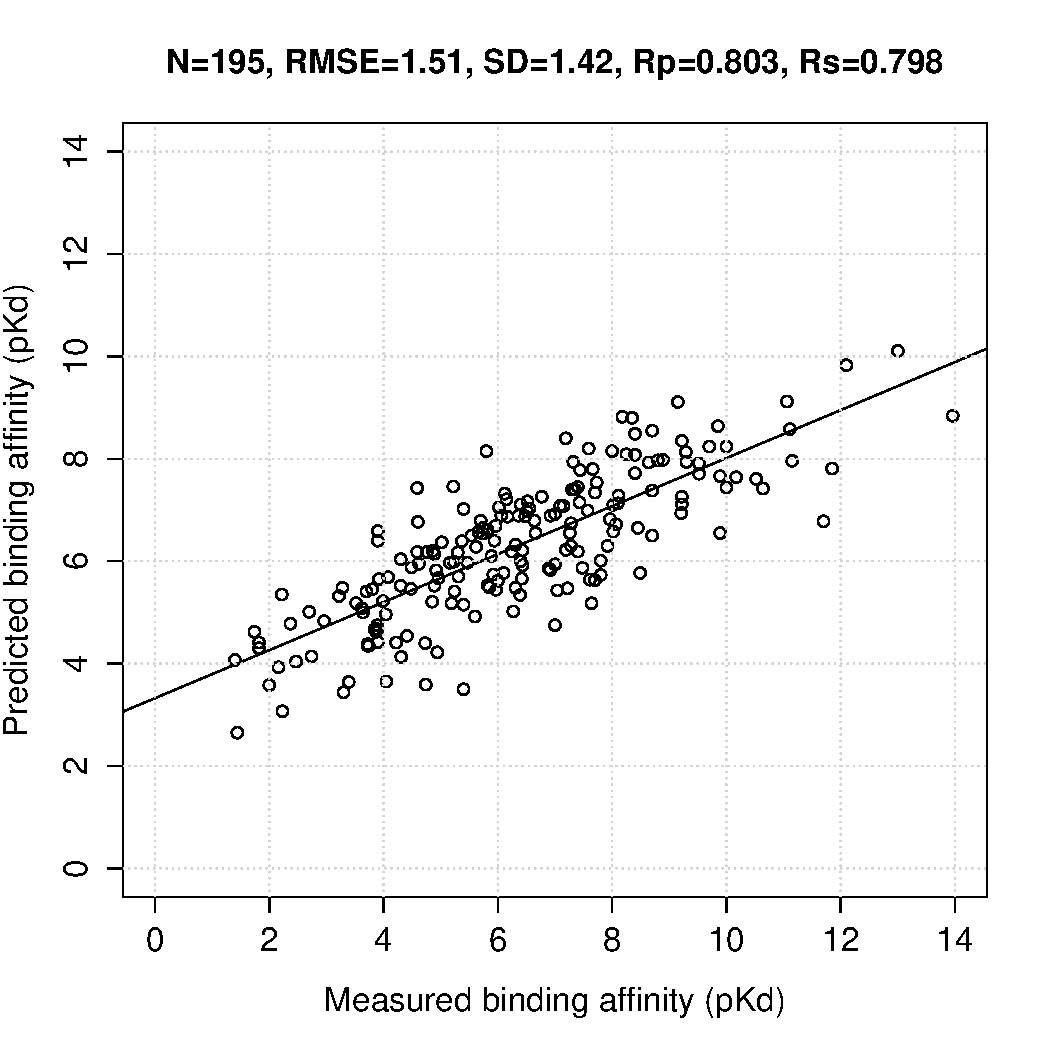
\includegraphics[width=0.48\linewidth]{../rfscore3/model-4-set-1-pdbbind-2007-tst-yp.pdf}
}
\caption{Performance on the 195 test set complexes in the PDBbind benchmark (partition 1 in Table \ref{rfscore3:partitions}).}
\label{rfscore3:partition1stat}
\end{figure}

Figure \ref{rfscore3:partition5stat} shows their performance on the 2013 blind benchmark, with RF::VinaElem also achieving a substantial improvement over Vina of -0.86 in RMSE, -0.37 in SD, +0.280 in Rp and +0.245 in Rs. While there is a significant decrease in performance for both SFs with respect to the PDBbind benchmark (compare Figures \ref{rfscore3:partition1stat} and \ref{rfscore3:partition5stat}), the relative performance of both SFs is similar on both benchmarks as it was anticipated \citep{908}. A linear regression model with molecular weight of the ligand as only variable was trained and tested on the sets and obtained RMSE=1.90, SD=1.90, Rp=0.269 and Rs=0.330.

\begin{figure}
\centering
\subfloat[AutoDock Vina.]
{
  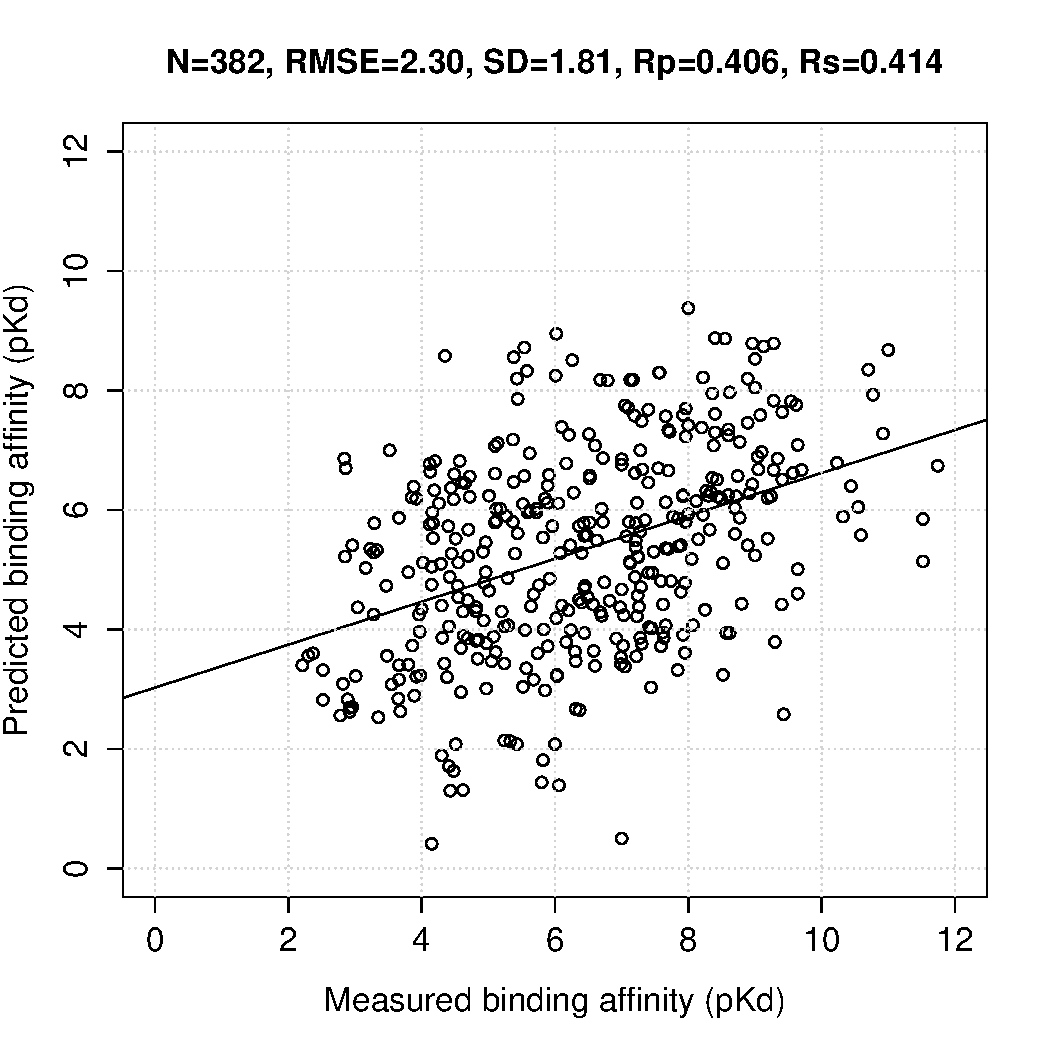
\includegraphics[width=0.48\linewidth]{../rfscore3/model-1-set-2-pdbbind-2007-tst-yp.pdf}
}
\subfloat[RF::VinaElem.]
{
  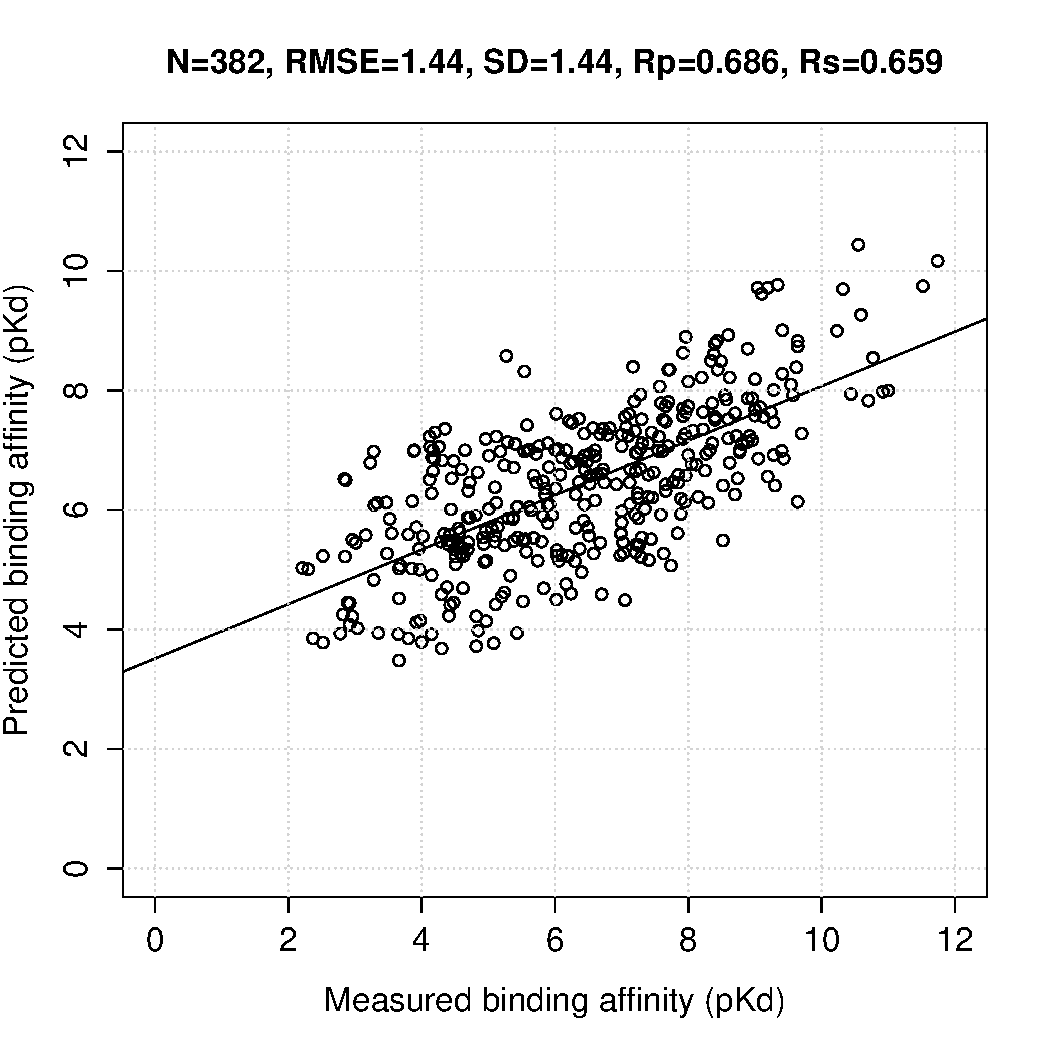
\includegraphics[width=0.48\linewidth]{../rfscore3/model-4-set-2-pdbbind-2012-tst-yp.pdf}
}
\caption{Performance on the 382 test set complexes in the 2013 blind benchmark (partition 5 in Table \ref{rfscore3:partitions}).}
\label{rfscore3:partition5stat}
\end{figure}

On the other hand, it is well known that there is a substantial correlation between ligand size and binding affinity. Thus, simple models such as the MWT baseline introduced in the previous subsection (see Table \ref{rfscore3:trn1105tst195}'s caption) have been used to put in perspective the performance of SFs. The performances compiled in Table \ref{rfscore3:trn1105tst195} show that many classical SFs are close to or even below this simple baseline (this is easier to see in Figure \ref{rfscore3:StandardDeviations}). By contrast, RF::VinaElem obtains an Rp of 0.803 on the PDBbind benchmark, which almost doubles that of MWT (0.418). On the 2013 blind benchmark, RF::VinaElem obtains a Rp of 0.686 whereas MWT's is just 0.269. This is not surprising as RF::VinaElem has been designed to learn the relation-ship between intermolecular interactions and binding affinity from structural data, not ligand properties. 

Overall, it is remarkable that RF::VinaElem achieves an error of just 1.44 pKd units, 1.96 kcal/mol, in a blind benchmark comprising such a diverse independent test set (see Figure \ref{rfscore3:partition5stat}). It would be interesting to see how well classical SFs perform on this benchmark, including those in Table \ref{rfscore3:trn1105tst195} (Vina's RMSE=2.30 translates to 3.14 kcal/mol) and even theoretically more accurate techniques such as free energy calculations (Michel and Essex, 2010).

\subsection{Machine-learning SFs assimilate data better than empirical SFs}

This subsection analyses the reasons why machine-learning SFs perform so well in predicting the binding affinities of diverse protein-ligand complexes. It also investigates how this performance improvement over classical SFs is expected to widen with the future availability of more training data. As explained in section 2.6, the 382 complexes appeared in 2013 are predicted with models trained on data up to 2002 (792 complexes in partition 2), 2007 (1300 complexes in partition 3), 2010 (2059 complexes in partition 4) and 2012 (2897 complexes in partition 5). 

Figure \ref{rfscore3:partitions2345SD} shows how the SD error in predicting pKd varies with training data size. RF-based SFs are represented by boxplots to show how their performance varies using 10 different random seeds for training on the same data (the other SFs are not stochastic and only a single performance value can be obtained from a particular training data set). The comparison between models 2 and 3 is particularly striking. The performance of model 2, effectively a classical SF, does not improve with training data set size. By contrast, model 3, whose only difference with model 2 is in using RF instead MLR as the regression model, greatly improves with more data. This demonstrates that the circumvention of an additive functional form is one of the reasons, further supporting the same conclusions on the PDBbind benchmark discussed in subsection 3.1.

\begin{figure}
\centering
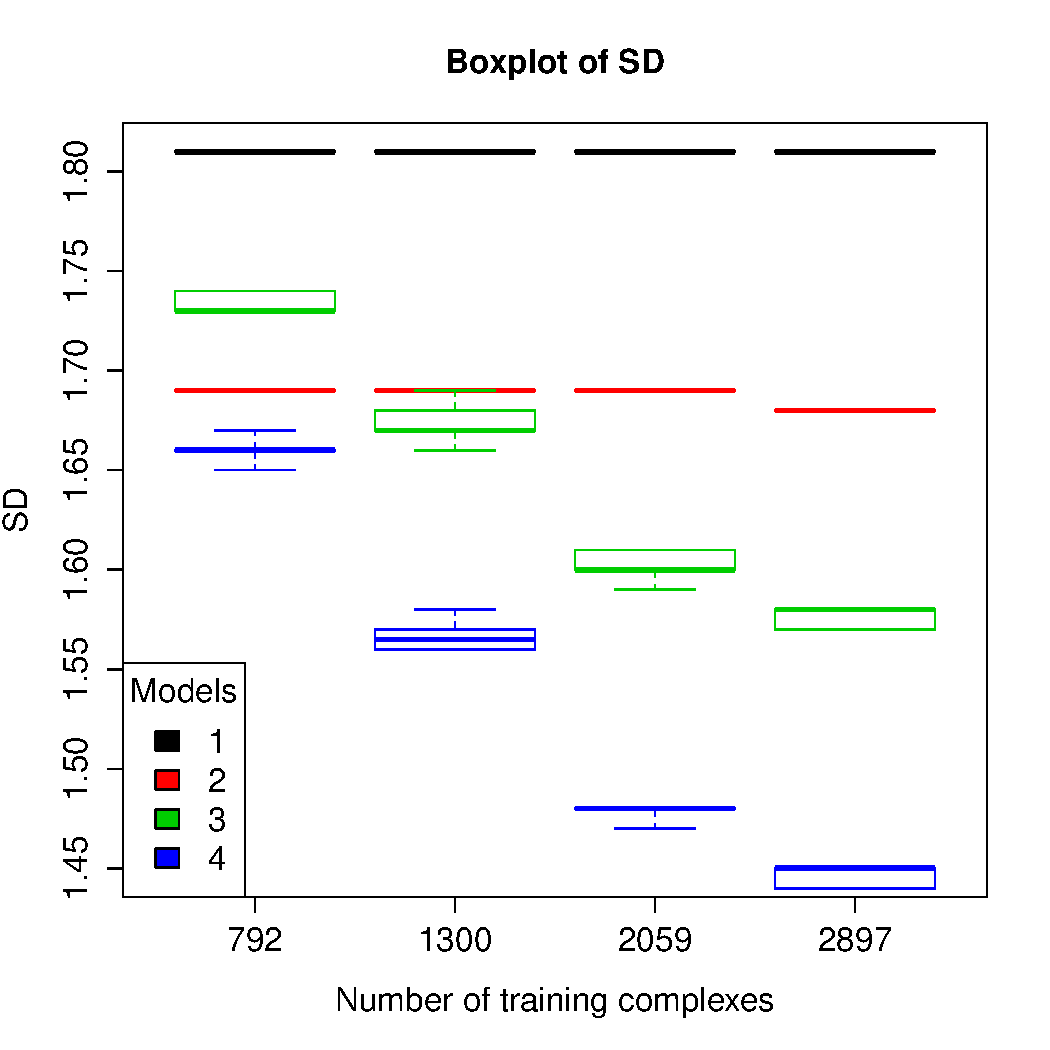
\includegraphics[width=\linewidth]{../rfscore3/set-2-tst-sdev-boxplot.pdf}
\caption{SD error in predicting binding affinities of the 382 new complexes in 2013 using the four SFs and four training sets formed by the complexes known in 2002, 2007, 2010 and 2012.}
\label{rfscore3:partitions2345SD}
\end{figure}

The second reason why machine-learning SFs perform so well is that RF is capable of effectively exploiting a more comprehensive set of structural features. This can be seen by comparing the performance of models 3 and 4, which only differ in that model 4 uses 36 features in addition to the six used by model 3. Again, not only the difference in performance is substantial but grows as more data is available for training, thus increasing the importance of using RF in the future.

Figure \ref{rfscore3:partitions2345RsRp} shows the correlations with binding affinity for the same numerical experiment (this time only the median is shown to better appreciate the trends from each model). The same conclusions are reached from this complementary view of performance: a non-parametric regression model performs better because it circumvents modelling assumptions and is capable of better exploiting richer structural descriptions of the complex. For the training set with the lowest number of complexes, model 2 outperforms model 3, suggesting that the additivity assumption of classical SFs was the best approach back in the days where few structures were available to calibrate the SF. It is also noteworthy that model 2 performs better than model 1, which suggests that the nonlinear OLS used in Vina is not as suitable as MLR, at least for this crucial aspect of docking. Note that model 1 represents the situation where a SF is used off-the-shelf without retraining for each set, although here we have seen that improvements with data set size can only be gained by using the appropriate regression model.

\begin{figure}
\centering
\subfloat[Rs.]
{
  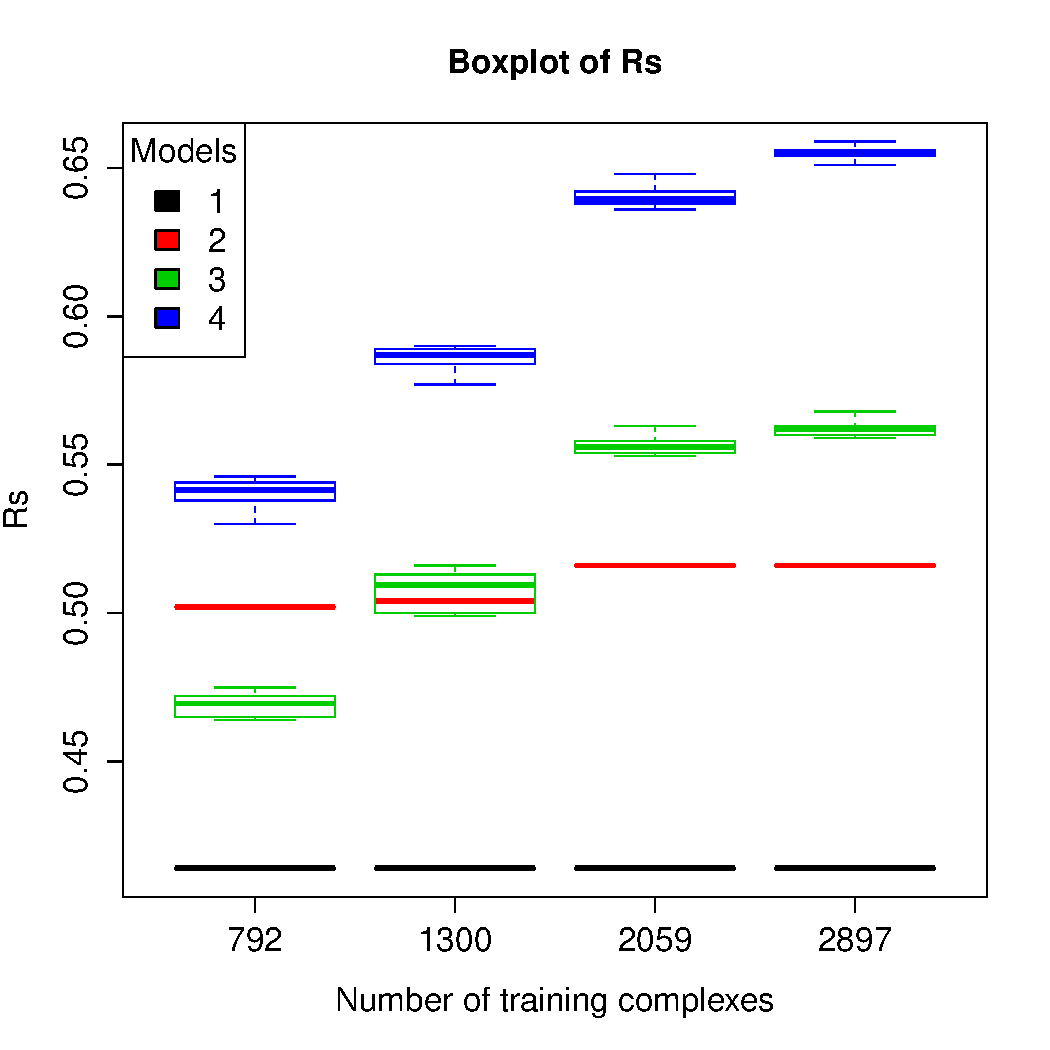
\includegraphics[width=0.48\linewidth]{../rfscore3/set-2-tst-scor-boxplot.pdf}
}
\subfloat[Rp.]
{
  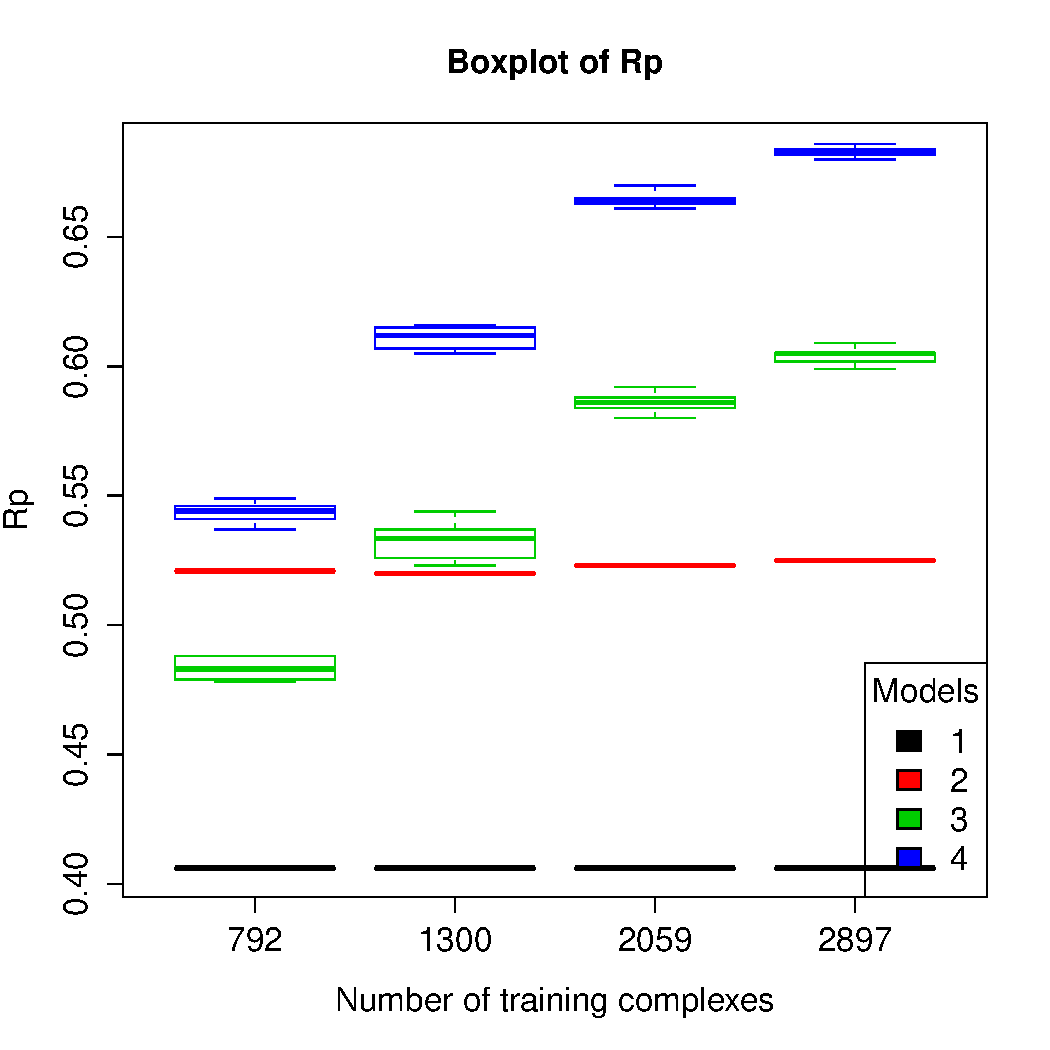
\includegraphics[width=0.48\linewidth]{../rfscore3/set-2-tst-pcor-boxplot.pdf}
}
\caption{Spearman rank-correlations (left plot) and Pearson correlations (right plot) with measured binding affinity on the 382 new complexes in 2013 using the same four SFs and training sets as in Figure 6.}
\label{rfscore3:partitions2345RsRp}
\end{figure}

\subsection{Machine-learning SFs can also be used to interpret docking results}

In addition to predicting binding affinity, the magnitude of the terms or features of a SF for a docking pose can be used to understand which the most important contributions to binding are. There are a number of ways in which this sensitivity analysis can be done. In a chemical series, one can look at how the value of each feature correlates with measured binding affinity, the more important for binding being those obtaining a higher correlation. For a particular docking pose, one can multiply each feature with its weight to obtain the energetic contribution to binding of each feature. Because knowledge-based SFs typically have no weights, it has been claimed \citep{1372} that these can hardly provide immediate physical interpretation of the results. In reality, one could also evaluate the SF for that pose with each feature set to zero in turn, with the features leading to the largest variation in the predicted pKd value being the most important. This can also be easily implemented in machine-learning SFs to understand ligand binding.

Another potential issue is that the set of features may not be directly related to intermolecular interactions. This is not the case of model 3, which has the same six directly interpretable features as model 2 representing an empirical SF. Nevertheless, model 4 incorporates 36 additional features which are not directly interpretable. Before assessing whether this is a drawback, we should remember what interpretability is ultimately useful for. Often, the optimisation of ligand potency is carried out by synthesising derivatives that pre-serve important favourable interactions and reduce unfavourable interactions according to such interpretation. However, extracting knowledge from a docking pose using a less accurate SF to use the derived knowledge to optimise ligand potency is clearly less accurate than simply using the most accurate SF to score all possible derivatives in order to synthesise those that are predicted to be more potent. Therefore, rather than a drawback, we believe that circumventing the interpretability stage can be an advantage in structure-based optimisation.

\subsection{The applicability domain of the developed SFs}

The applicability domain of a regression model is given by the set of training data points and how these are represented. Consequently, models 2 and 3 have the same applicability domain and thus are expected to work well on the same types of complexes (i.e. same types of molecules and proteins). Model 4 is trained and tested on the same data sets and thus should have a similar applicability do-main than models 2 and 3. However, since the data representation is different in that model 4 incorporates an additional set of features, the applicability domain will not be exactly the same. It is important to note that these features encode neither the chemical structure of the ligand nor the sequence information of the protein. Therefore, there is no reason to think that its applicability domain is more restricted to the chemotypes and protein families in the training set any more than other SFs trained on the same data are.

\section{Conclusions}

We have seen that one can greatly improve Vina by circumventing its assumed functional form using RF as the regression model and expanding the set of features describing the complexes. The resulting machine-learning SFs have either the same or very similar applicability domain by construction. Furthermore, we have explained how these SFs could be also used to understand binding. However, we have also argued that extracting knowledge from the description that a SF provides of a docking pose is a suboptimal way to improve ligand binding, as the direct application of a more accurate SF on ligand derivatives should perform better. Lastly, we have demonstrated that the tendency of RF-based SFs to overfit training data is not a limitation but simply a trait of these regression models which are robust to overfitting.

Given the large number of Vina users and the large increase in scoring accuracy achieved, we have trained the best of our models on the most comprehensive set of high-quality complexes (RF-Score-v3; RF::VinaElem trained on the 2959 complexes from 2013 refined set) and implemented it as easy-to-use software that directly re-scores Vina-generated poses (see the first page for availability and the README file therein for operating instructions).

Because classical SFs generally use MLR as the regression model and we have shown its inability to improve with larger volumes of structural data, we expect that the performance of any of these will be boosted by following the same procedure we have applied here to Vina. We therefore urge developers to modify their SFs accordingly so that users can enjoy a much higher accuracy. Using non-parametric machine learning remains a largely unexplored approach to developing SFs. For instance, the incorporation of ligand-only, protein-only and alternative intermolecular features, e.g. \citep{1303}, is still to be fully investigated. 

The proposed benchmark, effectively a blind test using four time-stamped training sets, has revealed that the performance difference between classical and machine-learning SFs will be larger as more structural data becomes publicly available in the future. The latter could include the very large number of experimentally-determined structures that are continuously generated by the pharmaceutical industry. Confidentiality should not be a problem, as only the inter-molecular features and binding affinities of these structures are required to improve SFs from which it is not possible to elucidate the identity of neither the targets nor the bound molecules. It is important to note that this is a new opportunity because, as we have shown here, the regression model adopted by classical SFs would not be able to exploit this new flood of data. 

As usual, e.g. \citep{1313}, the performance of generic SFs has been assessed by measuring their ability to predict the binding affinities of diverse protein-ligand complexes. Given its accuracy at this task, RF-Score-v3 should generally perform well on structure-based drug lead optimization applications. We have however not investigated its ability to discriminate between binders and non-binders (virtual screening; VS) yet, as it was important to study first binding affinity prediction in isolation, thus avoiding additional con-founding factors such as true binders that might not bind to the assumed binding conformation or pocket as well as assumed non-binders that might be actually binding. Since these issues are hence out the scope of this study, we are not making any claim about how RF-Score-v3 will compare to classical SFs on VS benchmarks. However, we expect that it will excel at VS because: (i) excellent prospective results have already been achieved with the less accurate RF-Score-v1 \citep{1281}, (ii) pose generation error has typically a low impact on binding affinity prediction \citep{1362}, (iii) accurate ranking by the affinity of true binders is a necessary condition for top VS performance, and (iv) non-binders are nothing but extremely weak binders whose low affinity should be best predicted by RF-Score-v3.

\section{Future works}

Enrichment
Protein-family specific scoring functions
Generate features from subsets of atoms, like UFSRAT and USRCAT.

\chapterend
